\documentclass[10pt,a4paper]{article}
\usepackage{titling}
\usepackage[margin=1 in]{geometry}
\usepackage{graphicx}
\graphicspath{{.}}
\newcommand{\subtitle}[1]{%
  \posttitle{%
    \par\end{center}
    \begin{center}\large#1\end{center}
    \vskip0.5em}%
}

\begin{document}

\title{\vspace{-3cm}Hot Protocol Version 1}
\subtitle{Hottentot RPC Framework}
\author{Kamran Amini}

\maketitle

\rule{15cm}{0.4pt}

\tableofcontents
\newpage

\section {Introduction}
This document talks about request and response structures and mechanisms in Hottentot RPC Framework. Purpose of this protocol is to convey Method Invocation request and response. Current protocol is serialization transparent and can convey a method call with arguments produced with different serialization algorithms. In this version, Hottentot's runtimes can only work with internal serialization mechanism.

\section {Glossary}
  \bigskip
  \textit {SERIALIZATION} \\ \indent {A process in which an object turns into a byte array to be transferred in a channel.} \\\\
  \textit {STRUCT} \\ \indent {A term used for encapsulation of fields related to a specific entity. It is a structure and  will be generated for each programming language differently.} \\\\
  \textit {IDL (INTERFACE DEFINITION LANGUAGE)} \\ \indent {An IDL is a language transparent to all programming languages which Hottentot supports. IDL can be generated to any target languages supported by Hottentot RPC Framework.} \\\\
  \textit {HOT FILE} \\ \indent {A file which contains IDL. Hot files usually end with \texttt{.hot} extension.} \\\\
  \textit {GENERATOR} \\ \indent {A tool for generating stub and struct source codes for a target programming language. Currently, generators for C++ and Java languages are available.} \\\\
  \textit {RUNTIME} \\ \indent {A library for a specific programming language which performs Service and Proxy operations. Currently, runtimes are only available for C++ and Java.} \\\\
  \textit {ENDPOINT} \\ \indent {Endpoint is a combination of IP address and a port. A service object is bound to an endpoint.} \\\\
  \textit {SERVICE} \\ \indent {Service is an object serving method invocation requests.} \\\\
  \textit {PROXY} \\ \indent {Proxy is an object which produces method invocation requests and receives the response. A proxy object directly talks to a service object.} \\\\

\section {Request}
A Method Invocation request consists of following fields:
\begin{itemize}
  \item Request Type (1 Byte)
  \item Service Id (4 Bytes)
  \item Method Id (4 Bytes)
  \item Number of Arguments (1 Byte)
  \item Arguments as an array of LV Structures. (Variable Length)
\end{itemize}

\begin{figure}[!ht]
  \caption{Structure of a Method Invocation request.}
  \centering
    \scalebox{2.1}{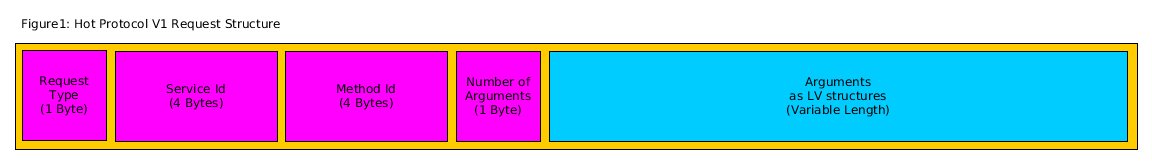
\includegraphics[width=0.5\textwidth]{hot-protocol-v1__figure1.png}}
\end{figure}

Figure 1 shows the structure of a request. Arguments can be transferred using LV structures. LV structures include Length and Value. Maximum length for a single LV structure is $2^{32} - 1$ since length values can be stored in a field at most 4 bytes. Figure 2 shows the LV structures in detail.

\begin{figure}[!ht]
  \caption{Structure of a Method Invocation request with arguments' LV structures.}
  \centering
    \scalebox{2.2}{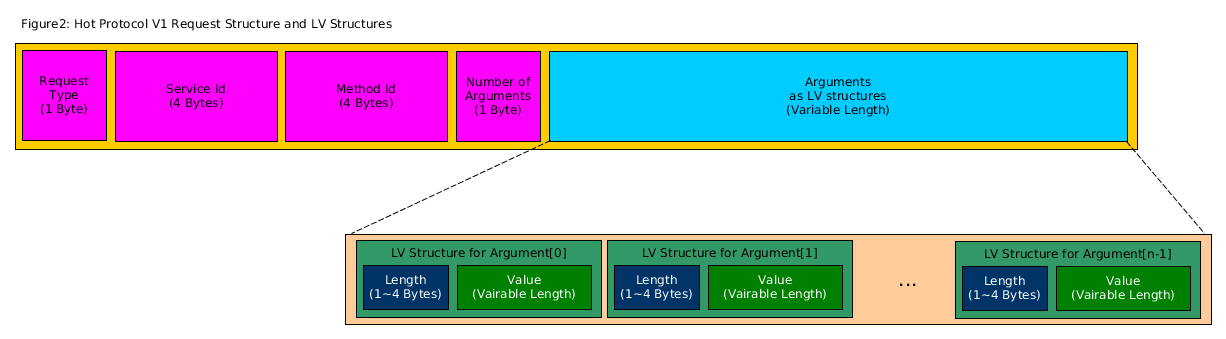
\includegraphics[width=0.5\textwidth]{hot-protocol-v1__figure2.png}}
\end{figure}

\section {Future Features}

\end{document}